%==============================================================================
% ModelCrew · CUMCM 国赛论文模板（中文，ctex，自包含）
%   编译：  latexmk -xelatex 6_paper.tex   （含中文，建议 XeLaTeX）
%   本文件由 Writer 据 templates/cumcm_paper_template.tex 填充占位符生成。
%   数字唯一真值源 = frozen_numbers.json，与 6_paper.md 同源。
%   注意：未在本机编译（如无 TeX 发行版，交付 .tex 源，请自行 xelatex 编译）。
%==============================================================================
\documentclass[12pt,a4paper]{ctexart}

\usepackage[margin=2.5cm]{geometry}
\usepackage{amsmath,amssymb}
\usepackage{graphicx}
\usepackage{booktabs}
\usepackage{titlesec}
\usepackage{abstract}
\usepackage[hidelinks]{hyperref}

\title{\textbf{冲突性校正的去冗余加权 TOPSIS 绿色低碳综合评价模型}}
\author{}
\date{}

\begin{document}

%------------------------------------------------------------------ 承诺页（占位）
\thispagestyle{empty}
\noindent 我们仔细阅读了竞赛章程与论文格式规范，承诺严格遵守，所提交论文为独立完成的研究成果，未抄袭、未泄露身份信息。（本段为占位，按当年官方诚信承诺书替换。）
\newpage

%------------------------------------------------------------------ 摘要页
\maketitle
\vspace{-2em}
\begin{center}\textbf{\large 摘\quad 要}\end{center}
\noindent
本文针对某省 10 个地区（A--J）在 7 项方向不一、量纲各异指标上的``绿色低碳发展水平''截面评价问题，建立一套\textbf{客观、可解释、字节级可复现}的多属性决策（MADM）综合评价模型，并以``赋权方法、指标口径、数据扰动''三轴稳健性如实界定其适用边界。

针对问题一（核心排序），将评价过程拆为``方向统一 $\rightarrow$ min-max 无量纲化 $\rightarrow$ 客观赋权 $\rightarrow$ 聚合排序''四段，主方案 \textbf{M1 采用 CRITIC 赋权 + 加权 TOPSIS}（命名为``冲突性校正的去冗余加权 TOPSIS''）。数据侦察发现 7 指标中存在一个``能源-碳-减排''强相关簇（\texttt{energy\_intensity} 与 \texttt{carbon\_intensity} 相关系数高达 +0.996，近共线），等权或熵权法会对该簇\textbf{重复计权}；CRITIC 借``对比强度 $\times$ 冲突性''使该簇 \texttt{energy+carbon} 权重和由单独标准差的 \textbf{0.2922} 被压到 \textbf{0.2261}（降约 24\%），并把权重转移给离散度高且最独立的 \texttt{forest\_cover}（权重 \textbf{0.2649}，全表最高）。最终排序为 \textbf{H > J > D > G > B > E > A > C > F > I}，第 1 名 H 贴近度 \textbf{0.7149}、垫底 I 仅 \textbf{0.1128}。

针对问题二（短板诊断），对 M1 末位三地区（C/F/I）用``SAW 缺口分解''与``TOPSIS 到正理想各维距离''双视角互证，三大短板完全一致：\textbf{C 为生态绿化+空气质量双弱}（森林覆盖 22\% 全省最低、PM2.5 偏高），\textbf{F 为全面落后}（可再生占比 12\%、固废利用 60\% 双低），\textbf{I 以 PM2.5=58 $\mu$g/m$^3$（全省最高）为头号硬伤}，据此给出对应到具体指标的可执行建议。

针对问题三（稳健性），瓶颈是\textbf{两条而非一条}：① 排名对\textbf{赋权方法}敏感，换整套赋权使 Spearman 降至 $\sim$0.68（PCA 因 $n=10$ 不稳，最分歧 0.3576），跨方法最不稳为 \textbf{C}（名次 2$\sim$8 翻动）；② 排名对\textbf{数据扰动}也不稳——用诚实的加性高斯噪声蒙特卡洛（固定种子，$n=1000$），仅 \textbf{5\%$\cdot$std 噪声即 77.0\% 的样本改变名次}，翻动集中在中段 \textbf{G/B/E}（B 在 72\% 样本中挪位）。但\textbf{头部 H/J/D 与尾部 A/C/F/I 双重稳健}（5\% 噪声下 0\% 翻动），故``H/J/D 居前、F/I 垫底''可作硬决策依据，中段应按``梯队''而非``逐名''处理。

\textbf{诚实加分点}：本文最初的乘性扰动实验因 min-max 对乘性缩放恒等（被完全抵消）而无效，识破后改用加性高斯噪声重做，才发现中段对噪声敏感——这一更正本身是稳健性分析诚实性的体现。

\vspace{1em}
\noindent\textbf{关键词：} CRITIC 赋权；加权 TOPSIS；去冗余综合评价；加性高斯噪声蒙特卡洛；绿色低碳

\newpage
\tableofcontents
\newpage

%------------------------------------------------------------------ 正文
\section{问题重述}

某省级主管部门需对下辖 10 个地区（A--J）的``绿色低碳发展水平''做一次综合评价，用于资源倾斜与考核排名。已采集每地区在 7 项指标上的最新统计值，含 3 项逆向（\texttt{energy\_intensity} 单位 GDP 能耗、\texttt{carbon\_intensity} 单位 GDP 碳排放、\texttt{pm25} PM2.5 浓度，越小越好）与 4 项正向（\texttt{renewable\_share} 可再生发电占比、\texttt{forest\_cover} 森林覆盖率、\texttt{solid\_waste\_util} 固废利用率、\texttt{park\_green\_percap} 人均公园绿地，越大越好）。数据为该轮评价\textbf{唯一给定输入}，无外部数据，要求方法客观、可解释、确定性、字节级可复现。

题面拆为三个子问题：

\begin{itemize}
\item \textbf{问题一（核心）}：建综合评价模型，对 A--J 排序，给完整名次、综合得分与排序依据，须交代方向统一、无量纲化与权重确定口径。
\item \textbf{问题二}：诊断排名靠后地区的\textbf{主要短板维度}（是哪些指标拖累），给\textbf{对应到具体指标的可执行}建议。
\item \textbf{问题三}：评估排序对\textbf{赋权方法、指标口径、数据扰动}的敏感性，点名最不稳地区，如实给出适用边界与局限。
\end{itemize}

本文路线：先做数据侦察识别陷阱（相关簇/离散度/极值），再以``四段管线''建主方案 M1 并保留 4 套对照，由对照群支撑问题三的多轴稳健性论证。

\section{问题分析与基本假设}

\subsection{问题分析}

本题是\textbf{小样本（$10\times7$）、无监督、全样本截面}的多属性决策评价，无标准答案、无总体抽样框架，因此：① ``绿色低碳水平''无官方量化定义，须由所选指标体系+赋权+聚合方式\textbf{操作化定义}；② $n=10$ 不能做统计推断，稳健性只能靠多方案与数据扰动的\textbf{敏感性分析}论证；③ 综合得分绝对值无外部物理意义，\textbf{以序数（名次）为主}，分差不可解释为倍率。

数据侦察暴露三个决定选型的事实：\textbf{D1 强相关簇（头号）}——方向统一后 \{\texttt{energy\_intensity}, \texttt{carbon\_intensity}, \texttt{renewable\_share}, \texttt{solid\_waste\_util}\} 四项两两 $|r|\geq0.88$，其中 \texttt{energy\_intensity}$\leftrightarrow$\texttt{carbon\_intensity} $r=+0.996$ 近共线，不去冗余会\textbf{重复计权}；\textbf{D2 离散度差异}——各列变异系数 CV 跨 0.137$\sim$0.462（3.4 倍），离散度驱动赋权会偏向高 CV 指标；\textbf{D3 极值敏感}——3 个温和离群（G renewable、H park、I pm25）会被 min-max 钉到 0/1。D1 直接决定主赋权法须能\textbf{显式去冗余}，是本题胜负手。

\subsection{基本假设（每条带理由与代价）}

\begin{itemize}
\item \textbf{A1} 7 项指标即``绿色低碳水平''的完备代理（题面指定其为唯一输入）——代价：缺经济/治理维度，综合得分有结构性盲区（写入局限）。
\item \textbf{A2} 10 地区横向可比，无须规模校正（多数指标已是强度/占比）——代价：个别隐含规模效应未校正会有偏。
\item \textbf{A3} 各指标在其方向上单调偏好、无饱和区（方向表只给单调正/逆）——代价：森林覆盖、人均绿地极端高值可能被高估。
\item \textbf{A4} 指标相关性可由 CRITIC 冲突性项显式处理——代价：权重受 $n=10$ 小样本相关估计噪声影响。
\item \textbf{A5} 数据真实无缺失、单位与题面一致（CSV $10\times7$ 满格无异常）。
\item \textbf{A6} 综合得分主要用于序数比较，分差解释须克制（无量纲化后得分无物理量纲）。
\item \textbf{A7} ``客观、可复现''优先于领域先验权重（题面明确要``客观''）——代价：纯客观可能与政策重要性脱节，用 M5 量化该张力。
\item \textbf{A8} $n=10$ 不做统计推断，稳健性靠扰动/多方案对照。
\end{itemize}

\section{符号说明}

\begin{center}
\begin{tabular}{cll}
\toprule
符号 & 含义 & 单位/范围 \\
\midrule
$X=(x_{ij})$ & 原始决策矩阵，行 $i\in\{A..J\}$、列 $j\in\{1..7\}$ & 各列原单位 \\
$r_{ij}$ & 方向统一+无量纲化后标准化值 & $[0,1]$ \\
$\sigma_j$ & 第 $j$ 列标准化后样本标准差（ddof=1） & --- \\
$R=(r_{jk})$ & 标准化后列间 Pearson 相关矩阵 & $[-1,1]$ \\
$C_j$ & CRITIC 信息量 = 对比强度 $\times$ 冲突性 & --- \\
$w_j$ & 第 $j$ 指标权重，$\sum_j w_j=1$ & $[0,1]$ \\
$v_{ij}=w_j r_{ij}$ & 加权标准化值 & --- \\
$v_j^+,\,v_j^-$ & 第 $j$ 列正/负理想值 & --- \\
$D_i^+,\,D_i^-$ & 地区 $i$ 到正/负理想解的加权欧氏距离 & --- \\
$C_i$ & 贴近度（综合得分），越大越好 & $[0,1]$ \\
\bottomrule
\end{tabular}
\end{center}

\section{模型的建立}

\subsection{四段评价管线}

设原始决策矩阵 $X\in\mathbb{R}^{10\times7}$，逆向集合 $\mathrm{Rev}=\{\texttt{energy\_intensity},\texttt{carbon\_intensity},\texttt{pm25}\}$。

\textbf{阶段 1+2 · 方向统一与无量纲化（同口径一次成型）。} 为杜绝``两处各自为政''的逻辑泄露，将逆向转正与 min-max 合并为同一步：
\begin{equation}
r_{ij}=
\begin{cases}
\dfrac{x_{ij}-\min_i x_{ij}}{\max_i x_{ij}-\min_i x_{ij}}, & j\notin\mathrm{Rev}\ (\text{正向})\\[2.2ex]
\dfrac{\max_i x_{ij}-x_{ij}}{\max_i x_{ij}-\min_i x_{ij}}, & j\in\mathrm{Rev}\ (\text{逆向})
\end{cases}
\end{equation}
如此 $r_{ij}\in[0,1]$，0 对应该列最差、1 对应最优，全部指标同向。

\textbf{阶段 3 · CRITIC 客观赋权（去冗余胜负手）。} 信息量 = 对比强度（标准差）$\times$ 冲突性（与其他指标不相关度之和）：
\begin{equation}
C_j=\sigma_j\sum_{k=1}^{7}\bigl(1-r_{jk}\bigr),\qquad
w_j=\frac{C_j}{\sum_{m=1}^{7}C_m}
\end{equation}
冲突性项 $\sum_k(1-r_{jk})$ 使强相关簇内指标（$1-r$ 小）自动被压权，正面处理 D1 重复计权，同时客观、数据导出，满足 A7。

\textbf{阶段 4 · 加权 TOPSIS 聚合排序。} 取 $v_{ij}=w_j r_{ij}$，正/负理想 $v_j^+=\max_i v_{ij}$、$v_j^-=\min_i v_{ij}$：
\begin{equation}
D_i^{\pm}=\sqrt{\sum_{j=1}^{7}\bigl(v_{ij}-v_j^{\pm}\bigr)^2},\qquad
C_i=\frac{D_i^-}{D_i^++D_i^-}
\end{equation}
$C_i$ 降序即排名。TOPSIS 对短板敏感，与问题二诊断天然衔接。我们将主方案命名为\textbf{``冲突性校正的去冗余加权 TOPSIS''}：式(2)冲突性项是``去冗余''来源，式(3)距离结构是``抗短板''来源。

\subsection{对照方案群（服务问题三）}

固定其余环节、单换一处：M0（min-max+等权+加权和，零信息基线）、M2（熵权+加权和，不去冗余反面镜子）、M3（PCA 主成分，去冗余独立验证）、M5（CRITIC$\times$政策先验+TOPSIS，A7 张力）；口径维度另用 N2（z-score）、N3（向量归一）替换 N1。

\section{模型的求解与结果}

\subsection{求解前置：PoC 冒烟闸（三判据全过）}

正式全量前先跑 $\leq30$ 行冒烟：① F 垫底（名次=9，PASS，验方向/口径自洽）；② G 或 H 居首梯队（H 名次=1，PASS）；③ CRITIC 对 D1 近共线对降权（\texttt{energy+carbon} 权重和 CRITIC 0.2261 < 单独标准差 0.2922，PASS，验冲突性项生效）。三条全过，进全量。

\subsection{问题一：CRITIC 权重与主排名}

\begin{table}[htbp]\centering
\caption{CRITIC 权重及相对等权（1/7=0.1429）增减}
\begin{tabular}{lccl}
\toprule
指标 & CRITIC 权重 & 相对等权增减 & 解读 \\
\midrule
\texttt{forest\_cover} & \textbf{0.2649} & \textbf{+0.1220} & 离散度高+独立，\textbf{唯一被抬高}的指标 \\
\texttt{pm25} & 0.1400 & $-0.0029$ & 相对等权\textbf{不升反微降} \\
\texttt{renewable\_share} & 0.1281 & $-0.0148$ & 簇内，被压 \\
\texttt{solid\_waste\_util} & 0.1253 & $-0.0176$ & 簇内，被压 \\
\texttt{park\_green\_percap} & 0.1157 & $-0.0272$ & 被压 \\
\texttt{energy\_intensity} & 0.1151 & $-0.0278$ & 簇内近共线，被压 \\
\texttt{carbon\_intensity} & \textbf{0.1110} & $-0.0319$ & \textbf{最低}：与 energy $r=0.996$，冲突性最小 \\
\bottomrule
\end{tabular}
\end{table}

由图~\ref{fig:weights} 可见，CRITIC 相对等权\textbf{唯一被抬高的是 \texttt{forest\_cover}（+0.1220）}，其余 6 项全被压；近共线对 \texttt{energy+carbon} 权重和由 0.2922 被压到 0.2261（降约 24\%），是 D1 从``风险''被处理为``已校正''的直接证据。

\begin{table}[htbp]\centering
\caption{M1 主排名（贴近度 $C_i$ 越大越好）}
\begin{tabular}{ccccc}
\toprule
名次 & 地区 & $C_i$ & $D^+$ & $D^-$ \\
\midrule
1 & \textbf{H} & \textbf{0.7149} & 0.1352 & 0.3392 \\
2 & \textbf{J} & \textbf{0.6650} & 0.1361 & 0.2702 \\
3 & \textbf{D} & \textbf{0.6039} & 0.1866 & 0.2845 \\
4 & G & 0.5349 & 0.2327 & 0.2676 \\
5 & B & 0.5294 & 0.2164 & 0.2434 \\
6 & E & 0.5282 & 0.1994 & 0.2232 \\
7 & A & 0.4609 & 0.2309 & 0.1974 \\
8 & C & 0.4239 & 0.2908 & 0.2140 \\
9 & \textbf{F} & \textbf{0.3166} & 0.3145 & 0.1457 \\
10 & \textbf{I} & \textbf{0.1128} & 0.3632 & 0.0462 \\
\bottomrule
\end{tabular}
\end{table}

\begin{figure}[htbp]\centering
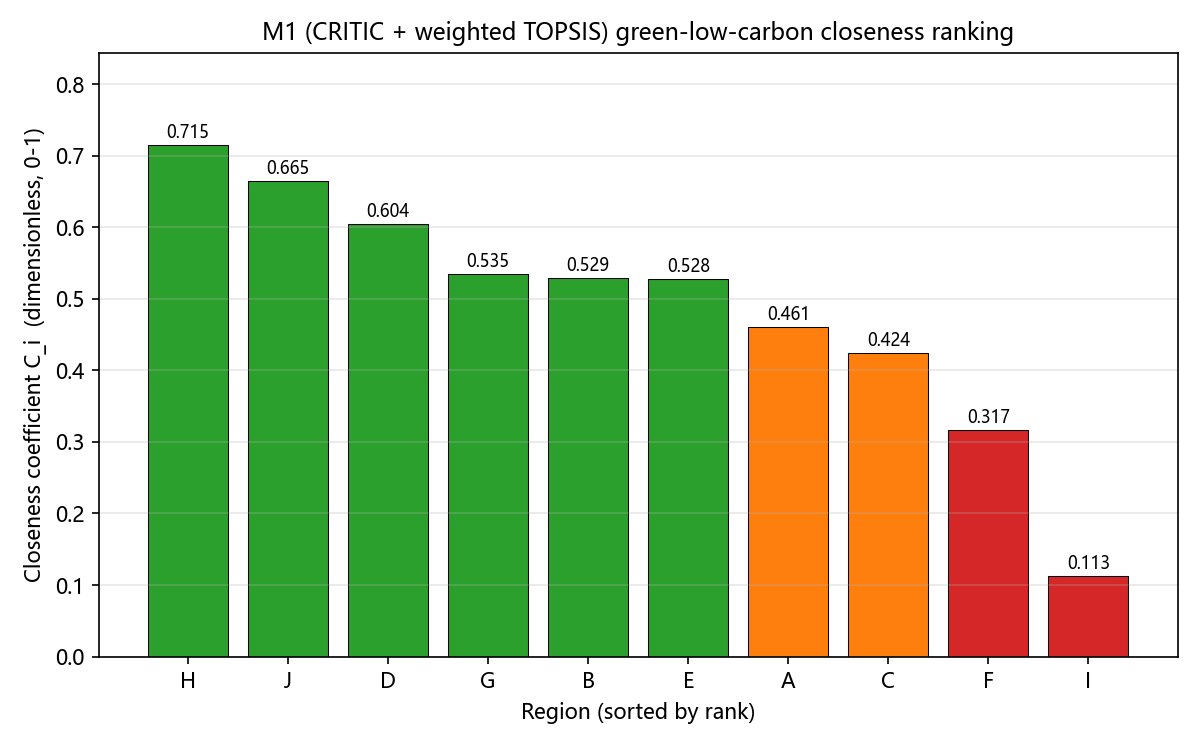
\includegraphics[width=0.85\textwidth]{figures/fig1_M1_ranking_bar.png}
\caption{M1（CRITIC + 加权 TOPSIS）各地区贴近度排名条形图}
\label{fig:rank}
\end{figure}

\begin{figure}[htbp]\centering
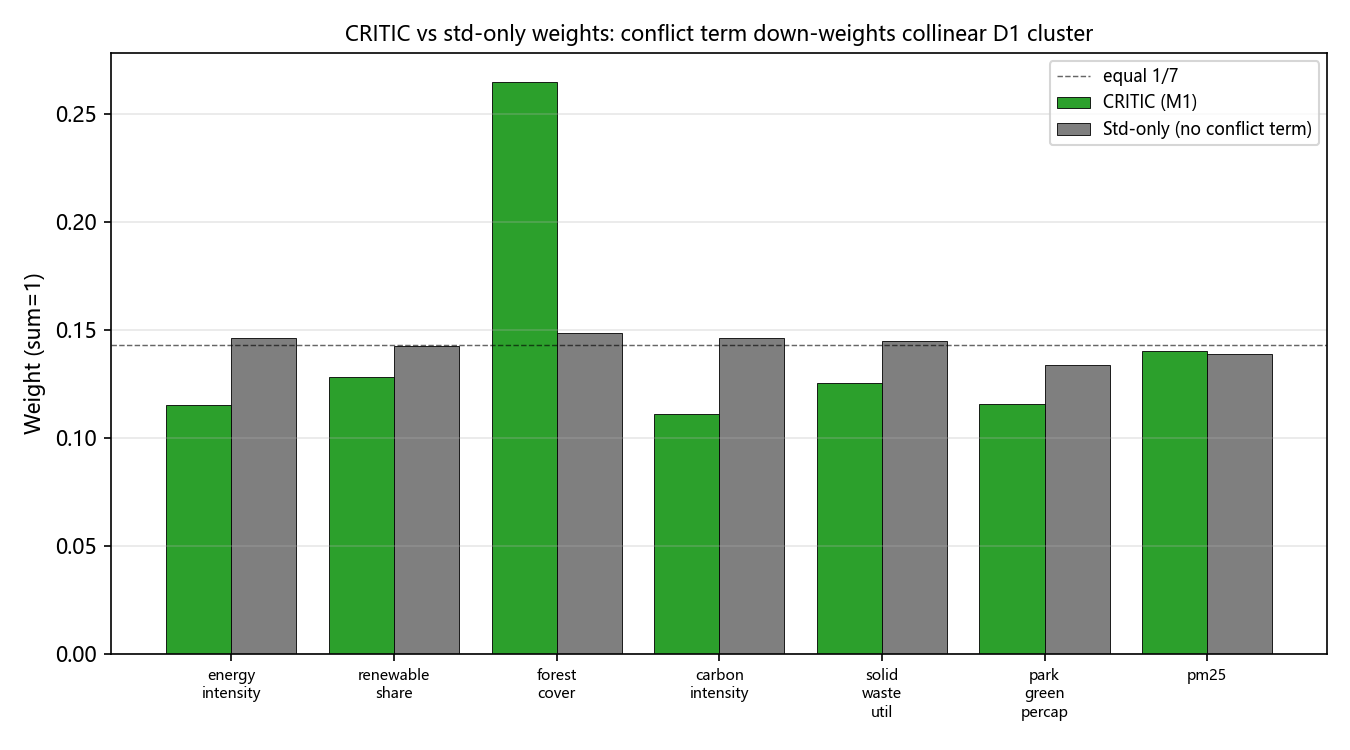
\includegraphics[width=0.85\textwidth]{figures/fig4_critic_vs_std_weights.png}
\caption{CRITIC 与单独标准差权重对比：冲突性项对 D1 强相关簇降权}
\label{fig:weights}
\end{figure}

排序结论：\textbf{H > J > D > G > B > E > A > C > F > I}，前三 H/J/D、垫底三 C/F/I。

\textbf{G 与 H 谁居首 $\rightarrow$ H（H=1，G=4）。} 这落在 D1 去冗余争议点上：G 在强相关簇 4 项全优，但 CRITIC 把该簇压权、把高离散度$\times$高冲突性的 \texttt{forest\_cover} 单独抬到 0.2649（相对等权 +0.1220，唯一被抬），而 H 的 \texttt{forest\_cover=70} 全省最高 $\rightarrow$ H 在被抬权的独立项上独大，反超 G。受控实验佐证：std-only / 等权下 G=1、H=3，唯有加入冲突性项才 H=1、G=4。故 H 反超\textbf{仅由 \texttt{forest\_cover} 抬权驱动，与 \texttt{pm25} 无关}（pm25 权重相对等权微降 $-0.0029$）。

\textbf{得分基数克制（A6）}：$C_i$ 仅供序数比较，B(0.5294) 与 E(0.5282) 仅差 \textbf{0.0012}，名次差不应解读为实质差距。

\subsection{问题二：靠后地区短板诊断}

门槛（出分后定）：M1 名次 $\geq$ 8，即末位三家 C/F/I。归因用 SAW 缺口分解 $w_j\cdot(1-r_{ij})$ 与 TOPSIS 到正理想各维距离$^2$ 双视角，两视角 top3 短板\textbf{完全一致}（互证，见图~\ref{fig:shortboard}）。

\begin{table}[htbp]\centering
\caption{末位三地区短板诊断（双视角互证）}
\begin{tabular}{ccll}
\toprule
地区 & 名次 & 三大短板（贡献降序） & 原始值（拖累维度） \\
\midrule
\textbf{C} & 8 & \texttt{forest\_cover}/\texttt{pm25}/\texttt{park\_green} & 森林 22\%(最低)·PM2.5 45·绿地 12.8 \\
\textbf{F} & 9 & \texttt{renewable}/\texttt{solid\_waste}/\texttt{forest} & 可再生 12\%(最低)·固废 60\%(最低)·森林 48\% \\
\textbf{I} & 10 & \texttt{forest\_cover}/\texttt{pm25}/\texttt{renewable} & 森林 26\%·PM2.5 58(最高)·可再生 17\% \\
\bottomrule
\end{tabular}
\end{table}

\begin{figure}[htbp]\centering
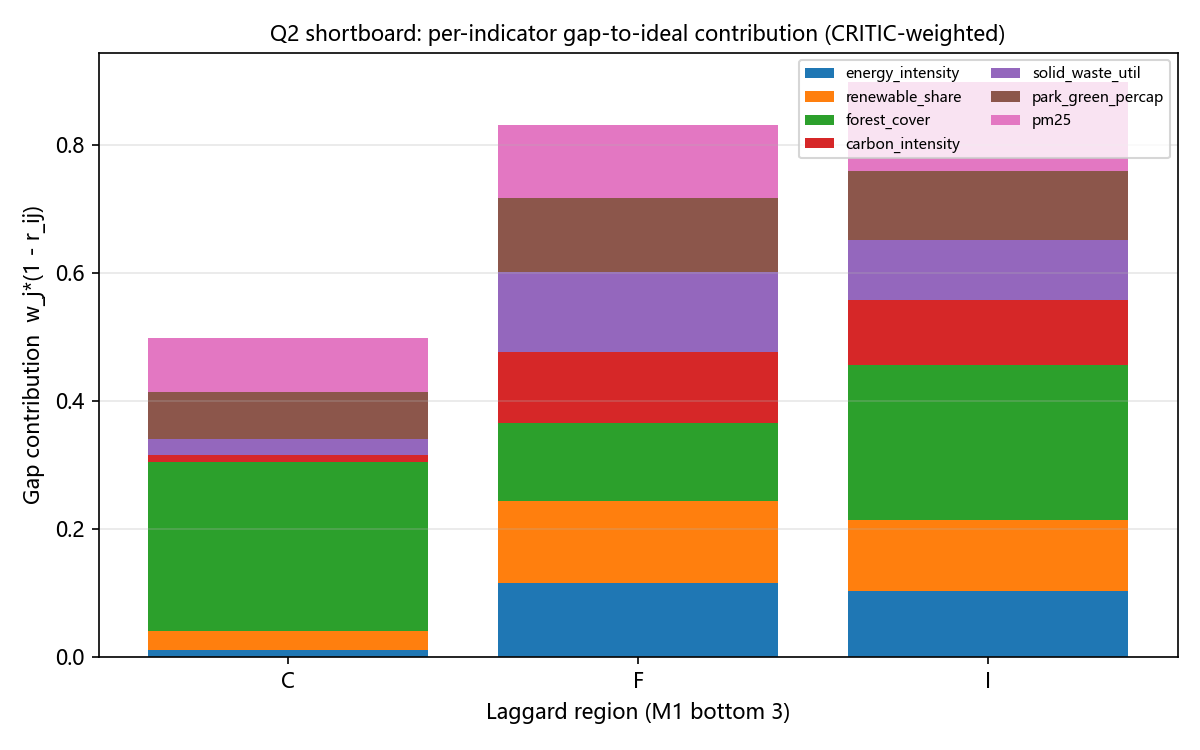
\includegraphics[width=0.8\textwidth]{figures/fig5_shortboard_diagnosis.png}
\caption{末位三地区各指标对得分缺口的 CRITIC 加权贡献堆叠图}
\label{fig:shortboard}
\end{figure}

\textbf{可执行建议（对应到指标，非空泛）}：\textbf{C}（生态绿化+空气质量双弱）以国土绿化/退耕还林提森林覆盖、建成区增公园绿地、联防联控降 PM2.5 为抓手，其能源指标尚可故评价分歧最大、名次须标注不确定性；\textbf{F}（全面落后）抓能源结构+固废循环，优先扩风光装机（现 12\%）、补固废产能（现 60\%）；\textbf{I}（PM2.5 头号硬伤）以 PM2.5 治理为牵引（产业/能源/交通协同减排），同步造林。

\section{灵敏度分析}

\subsection{赋权方法敏感性}

以 M1 为基准的秩相关：M5=0.7091、M0=0.6848、M2=0.6606、\textbf{M3 PCA=0.3576（最分歧）}。\textbf{去冗余单独效应（C2 受控隔离）}：M1 vs M2 同时换了赋权与聚合两个变量，是混杂对比；固定 TOPSIS 仅换权重时，CRITIC vs 熵权/等权/std-only 的 Spearman \textbf{均为 0.6848}。故应如实表述为``换整套赋权方案使 Spearman 降至 $\sim$0.68''，而这几乎全部来自 \texttt{forest\_cover} 被抬权，不应把混杂对比包装成纯去冗余因果。\textbf{PCA 局限}：M3 的 PC1 仅解释 \textbf{60.3\%} 方差、由能源簇主导，把 H 从第 1 压到第 6，故 PCA 在 $n=10$ 下不稳，仅作去冗余的独立验证。

\begin{figure}[htbp]\centering
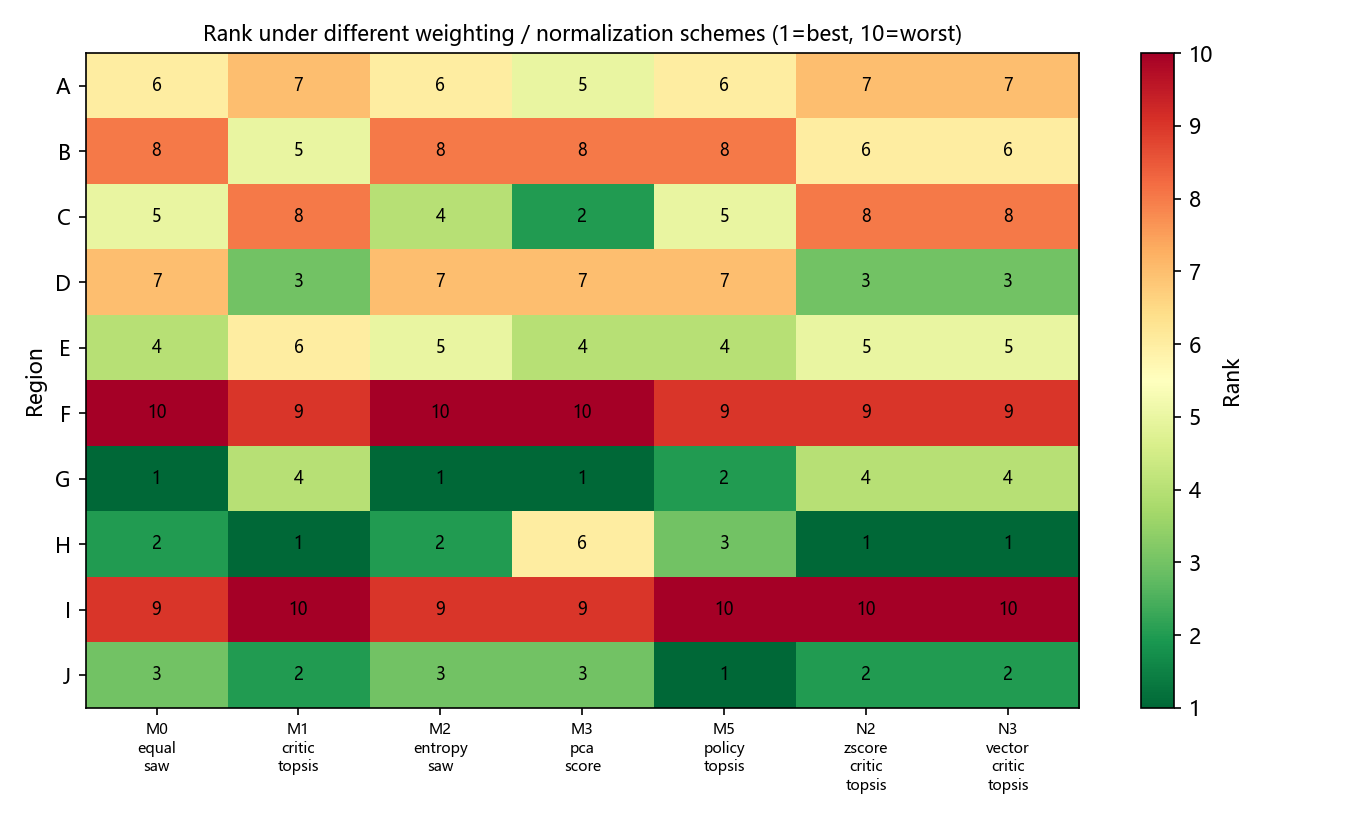
\includegraphics[width=0.92\textwidth]{figures/fig2_cross_method_rank_heatmap.png}
\caption{7 套赋权/口径方案下各地区名次热图（跨方法稳健性）}
\label{fig:heatmap}
\end{figure}

\subsection{无量纲化口径敏感性}

固定 CRITIC+TOPSIS，N2（z-score）与 N3（向量归一）对 N1（min-max）的 Spearman 均为 \textbf{0.9879}，仅个别相邻名次微调。\textbf{口径维度高度稳健}：D3 极值敏感在最终名次层面未造成翻动。

\subsection{数据扰动敏感性（加性高斯噪声蒙特卡洛）}

\textbf{方法学诚实更正}：最初用``单列乘性 $\pm\delta$''扰动得``$\pm50\%$ 零翻转''，但 min-max 对乘性缩放是恒等式
$\text{min-max}(a\cdot x)=\frac{ax-a\min}{a\max-a\min}=\text{min-max}(x)$，
缩放被完全抵消、名次恒不变，``零翻转''是恒等式而非稳健性。识破后改用加性高斯噪声 $x'=x+N(0,\,k\cdot\sigma_j)$，$k\in\{5\%,10\%,20\%\}$，各跑 1000 次（固定种子 \texttt{20240625}，字节级可复现），每次重算 M1。

整体名次改变比例：5\%$\cdot$std $\rightarrow$ \textbf{77.0\%}（770/1000）、10\% $\rightarrow$ 83.1\%、20\% $\rightarrow$ 93.1\%。各地区 5\% 档：头部 H/J/D 与尾部 A/C/F/I 全 \textbf{0\%} 翻动；中段 \textbf{G(45\%)/B(72\%)/E(57\%)} 在 [4,6] 间频繁互换（贴近度仅差 0.005$\sim$0.007）。

\begin{figure}[htbp]\centering
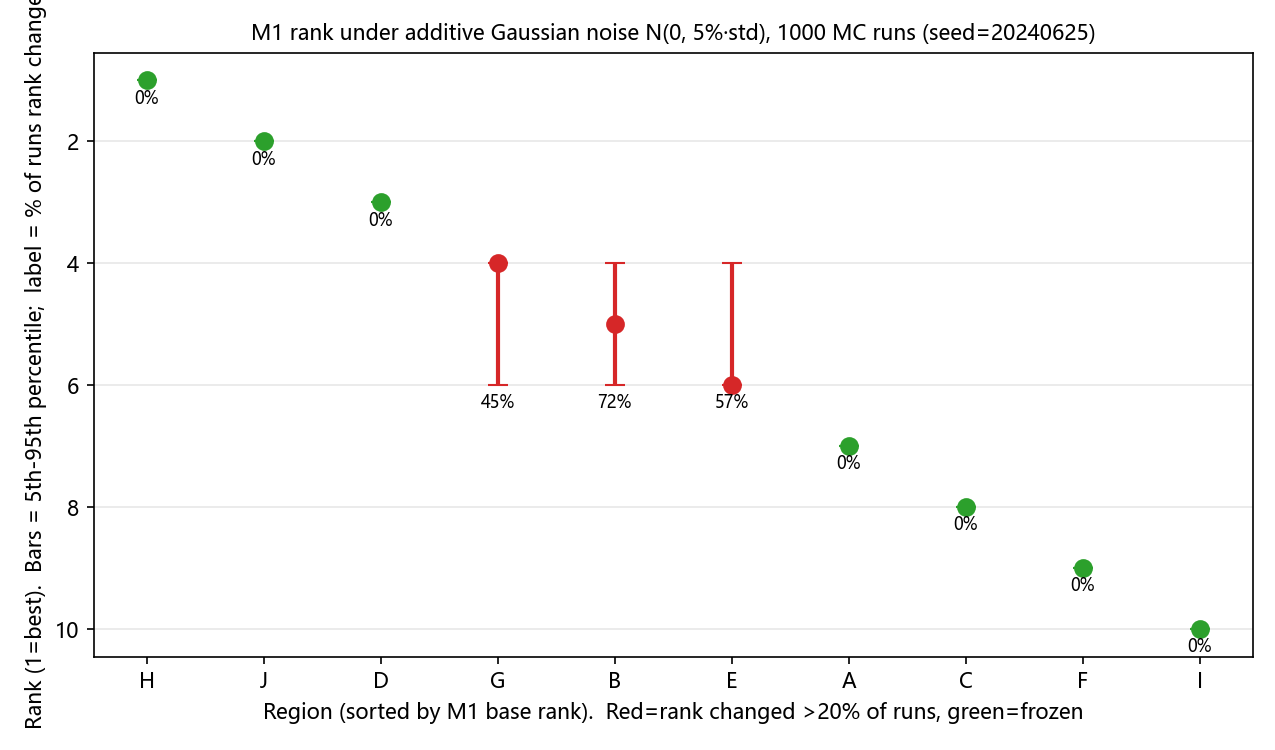
\includegraphics[width=0.85\textwidth]{figures/fig3_perturbation_rank_interval.png}
\caption{5\%$\cdot$std 加性高斯噪声下各地区名次 5--95 分位区间（红=翻动>20\%、绿=冻结，seed=20240625）}
\label{fig:perturb}
\end{figure}

故\textbf{排名对数据扰动并非``极稳''}，瓶颈是\textbf{两条}：既在赋权方法选择，也在数据噪声，均落于中段。

\subsection{最不稳地区点名（两类不稳互补）}

\textbf{跨方法最不稳=C}（名次 2$\sim$8，跨度 6）——M3 PCA 下第 2、CRITIC/熵权下第 8，是``用哪套权重决定命运''的典型，但对数据噪声反而稳（5\% 下 0\%），不稳来自赋权口径之争。\textbf{数据噪声最不稳=B}（72\% 样本改名次），E/G 次之，三家中段互换。\textbf{F、I 双重铁打垫底}（跨方法 9-10、5\% 噪声 0\% 翻动），同理头部 H/J/D 居前——这两端结论可作硬依据。

\section{模型的评价}

\subsection{优点}

\begin{enumerate}
\item \textbf{方法学针对性强、命名清晰}：``冲突性校正的去冗余加权 TOPSIS''用 CRITIC 冲突性项正面处理 D1（\texttt{energy+carbon} 权重和 0.2922$\rightarrow$0.2261，降约 24\%），是 5 套方案中唯一同时显式处理相关性冗余与离散度的客观法。
\item \textbf{全程客观可复现}：权重数据导出、无人为拍权；Q1/Q2/赋权口径敏感性确定性无随机，Q3 数据扰动用固定种子（20240625）MC，字节级可复现（\texttt{check\_frozen} 26/26 OK，Critic 独立重写代码复算 11 项关键数字逐位吻合）。
\item \textbf{诊断与建议闭环}：问题二双视角互证短板，建议逐条对应到具体指标。
\item \textbf{稳健性诚实且分层}：明确区分``头尾可硬决策、中段按梯队、C 标注不确定性''。
\end{enumerate}

\subsection{局限（如实写入审计结论）}

\begin{enumerate}
\item \textbf{稳健性瓶颈是两条而非一条}：排名既对赋权方法敏感（跨方法最不稳 C，跨度 6），也对数据扰动敏感（5\%$\cdot$std 噪声 77.0\% 样本改名次，中段 G/B/E 翻动）。\textbf{中段地区名次差仅千分位，在温和测量噪声下即频繁互换，其精确名次不可作硬决策依据}，应按``中段梯队''处理。
\item \textbf{一次方法学失误的诚实更正（加分而非掩盖）}：最初的乘性扰动因 min-max 恒等而无效，曾据此得``$\pm50\%$ 零翻转、瓶颈不在数据''的伪结论；识破后改用加性高斯噪声，才发现中段对噪声敏感，旧伪结论已撤回。主动暴露并修正这一弱点本身是稳健性分析诚实性的体现。
\item \textbf{指标体系不完备（A1）}：仅 7 项、无经济/治理维度，有结构性盲区——题目边界所限。
\item \textbf{单调偏好假设（A3）}：H 靠 forest=70/park=18.2 两个极值霸榜首位，其首位地位在单调假设下可能被高估。
\item \textbf{客观 vs 政策先验张力（A7）}：纯客观 CRITIC 把政策上更重要的碳指标赋了最低权（0.1110），M5 量化显示注入政策权重后排名翻动至 Spearman 0.7091——这是真实张力，已显式摆出而非隐藏。
\item \textbf{小样本 PCA 不稳}：PC1 仅解释 60.3\% 方差，对簇外优势地区低估，故仅作去冗余的独立验证。
\end{enumerate}

\subsection{改进方向}

引入\textbf{区间排序/聚类分层}把中段并为梯队输出区间名次（而非强行逐名，计算成本低、更贴合决策）；扩样本以救 PCA 与相关矩阵估计；按 M5 思路给碳/能耗设可调政策先验，向决策者提供``客观--政策''连续谱。

\section{结论}

本文建立``冲突性校正的去冗余加权 TOPSIS''绿色低碳综合评价模型，对 10 个地区给出客观、可解释、字节级可复现的排序 \textbf{H > J > D > G > B > E > A > C > F > I}（第 1 名 H 贴近度 0.7149、垫底 I 0.1128）。CRITIC 冲突性项把近共线``能源-碳''簇的权重和由 0.2922 压到 0.2261，并把权重转给最独立的 \texttt{forest\_cover}（0.2649），由此 H 反超 G。问题二诊断出 C（绿化+空气双弱）、F（全面落后）、I（PM2.5 头号硬伤）三家短板并给出对应指标的可执行建议。问题三经三轴敏感性如实界定边界：\textbf{``H/J/D 居前、F/I 垫底''双重稳健可作硬决策依据；中段 G/B/E 对赋权方法与 5\%$\cdot$std 数据噪声均敏感（77.0\% 样本改名次），应按梯队处理；C 的名次随赋权口径在 2$\sim$8 间翻动，须标注不确定性}。一次乘性扰动失效实验的诚实更正，亦体现本模型稳健性分析的可靠性。

\begin{thebibliography}{9}
\bibitem{critic} Diakoulaki D, Mavrotas G, Papayannakis L. Determining objective weights in multiple criteria problems: The CRITIC method[J]. Computers \& Operations Research, 1995, 22(7): 763-770.
\bibitem{topsis} Hwang C L, Yoon K. Multiple Attribute Decision Making: Methods and Applications[M]. Berlin: Springer-Verlag, 1981.
\bibitem{sikuikui} 司守奎, 孙玺菁. 数学建模算法与应用[M]. 北京: 国防工业出版社, 2015.
\bibitem{pca} Jolliffe I T. Principal Component Analysis[M]. 2nd ed. New York: Springer, 2002.
\end{thebibliography}

\appendix
\section{附录}

\textbf{求解脚本}：\texttt{artifacts/solve.py}（纯 Python；Q1/Q2/赋权口径敏感性确定性无随机，Q3 数据扰动用固定种子 \texttt{np.random.default\_rng(20240625)} 加性高斯噪声 MC，n=1000/档）。\textbf{输入}：\texttt{data/indicators.csv}（$10\times7$，未改动）。\textbf{输出}：\texttt{results.json}、\texttt{figures/fig1--fig5.png}。\textbf{真值源}：\texttt{frozen\_numbers.json}（26 项，\texttt{check\_frozen} $\rightarrow$ 26/26 OK）。\textbf{环境}：Python 3.14、numpy 2.4.2、pandas 3.0.2、matplotlib 3.10.8（Spearman/Kendall 手写实现）。\textbf{可复现保证}：固定列顺序；PCA 主成分符号显式校准（载荷和为正$\rightarrow$与``越大越好''同向）；数据扰动为固定种子加性高斯噪声，不再使用被 min-max 抵消的乘性扰动。

\end{document}
